\documentclass[letterpaper,11pt]{article}

\usepackage{latexsym}
\usepackage[empty]{fullpage}
\usepackage{titlesec}
\usepackage{marvosym}
\usepackage[usenames,dvipsnames]{color}
\usepackage{verbatim}
\usepackage{enumitem}
\usepackage[hidelinks]{hyperref}
\usepackage{fancyhdr}
\usepackage[english]{babel}
\usepackage{tabularx}
\usepackage{fontawesome5}
\usepackage{multicol}
\setlength{\multicolsep}{-3.0pt}
\setlength{\columnsep}{-1pt}
\input{glyphtounicode}

%new packages

\usepackage{fontenc}
\usepackage{amsmath}
\usepackage{amssymb}
\usepackage{graphicx}



%----------FONT OPTIONS----------

\pagestyle{fancy}
\fancyhf{} % clear all header and footer fields
\fancyfoot{}
\renewcommand{\headrulewidth}{0pt}
\renewcommand{\footrulewidth}{0pt}

% Adjust margins
\addtolength{\oddsidemargin}{-0.6in}
\addtolength{\evensidemargin}{-0.5in}
\addtolength{\textwidth}{1.19in}
\addtolength{\topmargin}{-.7in}
\addtolength{\textheight}{1.4in}

\urlstyle{same}

\raggedbottom
\raggedright
\setlength{\tabcolsep}{0in}

% Sections formatting
\titleformat{\section}{
  \vspace{-4pt}\scshape\raggedright\large\bfseries
}{}{0em}{}[\color{black}\titlerule \vspace{-5pt}]



% Ensure that generate pdf is machine readable/ATS parsable
\pdfgentounicode=1

%-------------------------
% Custom commands
\newcommand{\resumeItem}[1]{
  \item\small{
    {#1 \vspace{-2pt}}
  }
}

\newcommand{\classesList}[4]{
    \item\small{
        {#1 #2 #3 #4 \vspace{-2pt}}
  }
}

\newcommand{\resumeSubheading}[4]{
  \vspace{-2pt}\item
    \begin{tabular*}{1.0\textwidth}[t]{l@{\extracolsep{\fill}}r}
      \textbf{#1} & \textbf{\small #2} \\
      \textit{\small#3} & \textit{\small #4} \\
    \end{tabular*}\vspace{-7pt}
}

\newcommand{\resumeSubSubheading}[2]{
    \item
    \begin{tabular*}{0.97\textwidth}{l@{\extracolsep{\fill}}r}
      \textit{\small#1} & \textit{\small #2} \\
    \end{tabular*}\vspace{-7pt}
}

\newcommand{\resumeProjectHeading}[2]{
    \item
    \begin{tabular*}{1.001\textwidth}{l@{\extracolsep{\fill}}r}
      \small#1 & \textbf{\small #2}\\
    \end{tabular*}\vspace{-7pt}
}


\newcommand{\resumeSubItem}[1]{\resumeItem{#1}\vspace{-4pt}}

\renewcommand\labelitemi{$\vcenter{\hbox{\tiny$\bullet$}}$}
\renewcommand\labelitemii{$\vcenter{\hbox{\tiny$\bullet$}}$}

\newcommand{\resumeSubHeadingListStart}{\begin{itemize}[leftmargin=0.0in, label={}]}
\newcommand{\resumeSubHeadingListEnd}{\end{itemize}}
\newcommand{\resumeItemListStart}{\begin{itemize}}
\newcommand{\resumeItemListEnd}{\end{itemize}\vspace{-5pt}}

\begin{document}
\fontfamily{cmr}\selectfont
\begin{center}
\parbox{3.0cm}{%
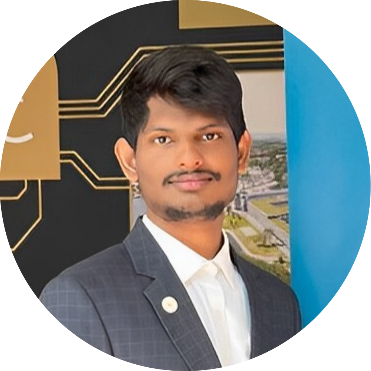
\includegraphics[width=2.7cm,clip]{images/resume_pic_m.png}}
}
\parbox{\dimexpr\linewidth-3.8cm\relax}{
\vspace{-20pt}
\begin{tabularx}{\linewidth}{L r} \\
    {\Huge \scshape  Venkata Sai Yakkshit Reddy Asodi}~
    \href{https://www.cedzlabs.com/yakkshit}{\vspace{1pt}}\\
      Berlin, Germany. \\ \vspace{1pt}
     \small \raisebox{-0.1\height}\faPhone\ +91 8179936156 ~ \href{mailto:saiyakkshit2001@gmail.com}{\raisebox{-0.2\height}\faEnvelope\  {saiyakkshit2001@gmail.com}} ~ 
    \href{https://linkedin.com/in/yakkshit/}{\raisebox{-0.2\height}\faLinkedin\ {yakkshit}}  ~
    \href{https://yakkshit.com/}{\raisebox{-0.2\height}\faGlobe\ {yakkshit.com}}  ~
    \href{https://github.com/yakkshit}{\raisebox{-0.2\height}\faGithub{ yakkshit}}
    \vspace{-8pt}
    
\end{tabularx}
}
\end{center}

%-----------SUMMARY-----------
\section{Summary}
Results-oriented Software Engineer specializing in building scalable, AI-driven systems. Expertise in Python, JavaScript frameworks, and cloud-based distributed architectures. Proven ability to design and deploy production-ready applications, with a focus on optimizing performance and creating user-friendly interfaces.

%-----------TECHNICAL SKILLS-----------
\section{Technical Skills}
\begin{itemize}[leftmargin=0.15in, label={}]
\small{
\item \textbf{Languages:} Python, JavaScript, SQL
\item \textbf{Frameworks:} React, Vue.js, Django
\item \textbf{Tools:} Git, Docker, AWS, SQLAlchemy, Pandas
\item \textbf{Deployment:} Kubernetes, Microservices, Azure
}
\end{itemize}

%-----------EXPERIENCE-----------
\section{Experience}

\textbf{Circleup AG} \hfill \textit{December 2023 -- July 2024} \\
Lead Full Stack Engineer (Frontend Focus) \hfill \textit{Zurich, Switzerland}
\begin{itemize}
    \item Developed responsive web applications using React and Django, focusing on API integrations and scalable architectures.
    \item Led front-end UI/UX design, implemented reusable components, and optimized application performance.
\end{itemize}

\textbf{Cedzlabs} \hfill \textit{March 2023 -- July 2024} \\
Full Stack Developer \hfill \textit{India}
\begin{itemize}
    \item Designed intuitive UIs with React and collaborated on cross-functional teams to deliver projects on time.
\end{itemize}

%-----------PROJECTS-----------
\section{Projects}
\textbf{AI Resume Tuner} | Azure, Next.js, RAG, LLMs \hfill \textit{August 2023}\\
\begin{itemize}
    \item Built an AI-driven resume generator for creating customized resumes, utilizing Retrieval Augmented Generation (RAG) and LLMs. Developed frontend with Next.js and deployed on Azure for scalability.
\end{itemize}

\textbf{Portfolio Website} | NextJS, AWS \hfill \textit{January 2023}\\
\begin{itemize}
    \item Created a personal website with a secure file encryption system, deployed on AWS with Next.js.
\end{itemize}

%-----------LANGUAGES-----------
\section{Languages}
\begin{itemize}
  \item Telugu - Native | English - Fluent | Hindi - Fluent | German - Elementary
\end{itemize}

%-----------ACHIEVEMENTS-----------
\section{Achievements / Extracurricular}
\begin{itemize}
    \item Implemented Agile methodologies in teams, actively contributed to open-source projects.
    \item Attended tech meetups on UI/UX and AI development.
\end{itemize}

%-----------STRENGTHS-----------
\textbf{Strengths:} Leadership, attention to detail, adaptability, and problem-solving.
\end{document}